\documentclass[]{article}
\usepackage{amsmath}
\usepackage{amssymb}
\usepackage{amsthm}
\usepackage[T1]{fontenc}
\usepackage{indentfirst}
\usepackage{tikz}
\usepackage{tipa}
\usetikzlibrary{arrows,automata}
\begin{document}

\title{COMS W3261 \\ Computer Science Theory \\ Chapter 3 Notes}
\author{Alexander Roth}
\date{2014--09--09}
\maketitle
\newtheorem{thm}{Theorem}

\section*{Regular Expressions}
  Regular expressions can define exactly the same languages that the various
  forms of automata describe: the regular languages. However, regular
  expressions offer something that automata do not: a declarative way to express
  the strings we want to accept. Thus regular expressions serve as the input
  language for many systems that process strings.

  \subsection*{The Operators of Regular Expressions}
    Regular expressions denote languages. There are three operations on
    languages that the operators of regular expressions represent. These
    operators are:
    \begin{enumerate}
      \item The \emph{union} of two languages $L$ and $M$, denoted by
      $L \cup M$, is the set of strings that are in either $L$ or $M$ or both.
      \item The \emph{concatenation} of languages $L$ and $M$ is the set of
      strings that can be formed by taking any string in $L$ and concatenating
      it with any string in $M$. The concatenation operator is frequently called
      ``dot''.
      \item The \emph{closure} (or \emph{star}, or \emph{Kleene closure}) of a
      language $L$ is denoted $L^*$ and represents the set of those strings that
      can be formed by taking any number of strings from $L$, possibly with
      repetitions and concatenating all of them.
    \end{enumerate}

\section*{Finite Automata and Regular Expressions}
  While the regular-expression approach to describing languages is fundamentally
  different from the finite-automaton approach, these two notations turn out to
  represent exactly the same set of languages, which we have termed the
  ``regular languages''. In order to show that the regular expressions define
  the same class, we must show that:
  \begin{enumerate}
    \item Every language defined by one of these automata is also defined by a
    regular expression. For this proof, we can assume the language is accepted
    by some DFA.
    \item Every language defined by a regular expression is defined by one of
    these automata. For this part of the proof the easiest is to show that there
    is an NFA with $\epsilon$-transitions accepting the same language. \\
  \end{enumerate}

  \subsection*{From DFA's to Regular Expressions}
    The construction of a regular expression to define the language of any DFA
    is surprisingly tricky. Roughly, we build expressions that describe sets of
    strings that label certain paths in the DFA's transition diagram. However,
    the paths are allowed to pass through only a limited subset of states.
    \begin{thm}
      If $L = L(A)$ for some DFA $A$, then there is a regular expression $R$
      such that $L = L(R)$.
    \end{thm}

  \subsection*{Converting DFA's to Regular Expressions by Eliminating States}
    The construction of a regular expression is expensive. Not only do we have
    to construct about $n^3$ expressions for an $n$-state automaton, but the
    length of the expression can grow by a factor of 4 on the average, with each
    of the $n$ inductive steps., if there is no simplification of the
    expressions. Thus, the expressions themselves could reach on the order of
    $4^n$ symbols. \\
    \indent The approach to constructing regular expressions that we shall now
    learn involves eliminating states. When we eliminate a state $s$, all the
    paths that went through $s$ no longer exist in the automaton. If the
    language of the automaton is not to change, we must include, on an arc that
    goes directly from $q$ to $p$, the labels of paths that went from state $q$
    to $p$, through $s$. Since the label of this arc may now involve strings,
    rather than single symbols, and the label of there may even be an infinite
    number of such strings, we cannot simply list the strings as a label.
    Fortunately, there is a simple, finite way to represent all such strings:
    use a regular expression. \\
    \indent Thus, we are led to consider automata that have regular expressions
    as labels. The language of the automaton is the union over all paths from
    the start state to an accepting state of the language formed by
    concatenating the languages of the regular expressions along that path. Each
    symbol $a$, or $\epsilon$ if it is allowed, can be thought of as a regular
    expression whose language is a single string, either $\{a\}$ or $\{\epsilon
    \}$. \\
    \indent We suppose that the automaton of which $s$ is a state has
    predecessors states $q_1, q_2, \ldots, q_k$ for $s$ and successor states
    $p_1,p_2,\ldots,p_m$ for $s$. It is possible that some of the $q$'s are also
    $p$'s, but we assume that $s$ is not among the $q$'s or $p$'s, even if there
    is a loop from $s$ to itself. We also show a regular expression on each arc
    from one of the $q$'s to $s$; expression $Q_i$ labels the arc from $q_i$.
    Likewise, we show a regular expression $P_i$ labeling the arc from $s$ to
    $p_i$, for all $i$. We show a loop on $s$ with label $S$. Finally, there is
    a regular expression $R_{ij}$ on the arc from $q_i$ to $p_j$, for all $i$
    and $j$. Note that some of these arcs may not exist in the automaton, in
    which case we take the expression on that arc to be $\emptyset$. \\
    \indent All arcs involving state $s$ are deleted. To compensate, we
    introduce, for each predecessor $q_i$ of $s$ and each successor $p_j$ of
    $s$, a regular expression that represents all the paths that start at $q_i$,
    go to $s$, perhaps loop around $s$ zero or more times, and finally go to
    $p_j$. The expression for these paths is $Q_iS^*P_j$. This expression is
    added (with the union operator) to the arc from $q_i$ to $p_j$. If there was
    no arc $q_i \rightarrow p_j$, then first introduce one with regular
    expression $\emptyset$. \\
    \indent The strategy for constructing a regular expression from a finite
    automaton is as follows:
      \begin{enumerate}
        \item For each accepting state $q$, apply the above reduction process to
        produce an equivalent automaton with regular-expression labels on the
        arcs. Eliminate all states except $q$ and the start state $q_0$.
        \item If $q \neq q_0$, then we shall be left with a two-state automaton
        that looks like this:

          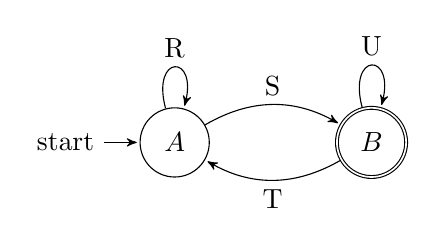
\begin{tikzpicture}[>=stealth',shorten >=1pt,auto,node distance=2.5cm]
            \node[initial,state]   (A)              {$A$};
            \node[state,accepting] (B) [right of=A] {$B$};

            \path[->] (A) edge [loop above] node {R} (A);
            \path[->] (A) edge [bend left]  node {S} (B);
            \path[->] (B) edge [bend left]  node {T} (A);
            \path[->] (B) edge [loop above] node {U} (B);

          \end{tikzpicture} \\

        The regular expression for the accepted strings can be described in
        various ways. One is $(R + SU^*T)^*SU^*$. In explanation, we can go from
        the state state to itself any number of times, by following a sequence
        of paths whose labels are in either $L(R)$ or $L(SU^*T)$. The expression
        $SU^*T$ represents paths that go to accepting state via a path in
        $L(S)$, perhaps return to the accepting state several times using a
        sequence of paths with labels in $L(U)$, and then return to the start
        state with a path whose label is in $L(T)$. Then we must go to the
        accepting state, never to return to the start state, by following a path
        with a label in $L(S)$. Once in the accepting state, we can return to it
        as many times as we like, by following a path whose label is in $L(U)$.
        \item If the start state is also an accepting state, then we must also
        perform a state-elimination from the original automaton that gets rid of
        every state but the start state. That will look something like this:

          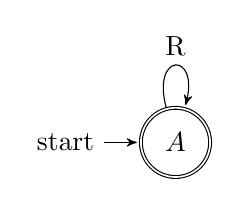
\begin{tikzpicture}[>=stealth',shorten >=1pt,auto,node distance=2.5cm]
            \node[initial,state,accepting] (A) {$A$};

            \path[->] (A) edge [loop above] node {R} (A);
          \end{tikzpicture} \\

        The regular expression denoting the strings that it accepts is $R^*$.
        \item The desired regular expression is the sum (union) of all the
        expressions derived from the reduced automata for each accepting state,
        by rules (2) and (3).
      \end{enumerate}

  \subsection*{Converting Regular Expresions to Automata}
    Every language $L$, that is $L(R)$ for some regular expression $R$, is also
    $L(E)$ for some $\epsilon$-NFA $E$. The proof is a structural induction on
    the expression $R$. We start by showing how to construct automata for the
    basis expressions: single symbols, $\epsilon$, and $\emptyset$. We then show
    how to combine these automata into larger automata that accept the union,
    concatenation, or closure of the language accepted by smaller automata.

    \subsubsection*{Ordering the Elimination of States}
      When a state is neither the start state nor an accepting state, it gets
      eliminated in all the derived automata. Thus, one of the advantages of the
      state-elimination process compared with the mechanical generation of
      regular-expressions is that we can start by eliminating all the states
      that are neither start nor accepting, once and for all. We only have to
      begin duplicating the reduction effort when we need to eliminate some
      accepting states.

    \begin{thm}
      Every language defined by a regular expression is also defined by a finite
      automaton.
    \end{thm}

\section*{Applications of Regular Expressions}
  We shall consider two important classes of regular-expression-based
  applications: lexical analyzers and text search.

  \subsection*{Regular Expressions in UNIX}
    Before seeing the applications, we shall introduce the UNIX notation for
    extended regular expressions. This notation gives us a number of additional
    capabilities. In fact, the UNIX extensions include certain features,
    especially the ability to name and refer to previous strings that have
    matched a pattern, that actually allow nonregular languages to be
    recognized. \\
    \indent The first enhancement to the regular-expression notation concerns
    the fact that most real applications deal with the ASCII character set. UNIX
    regular expressions allow us to write \emph{character classes} to represent
    large sets of characters as succinctly as possible. The rules for character
    classes are:
      \begin{itemize}
        \item The symbol \texttt{.} (dot) stands for ``any character''.
        \item The sequence $[a_1a_2\cdot{}a_k]$ stands for the regular
        expression

          \[ a_1 + a_2 + \cdots + a_k \]

        The notation saves about half the characters, since we don't have to
        write the $+-$ signs. For example, we could express the four characters
        used in C comparison operators by \texttt{[<>=!]}.
        \item Between the square braces we can put a range of the form
        \emph{x-y} to mean all the characters from $x$ to $y$ in the ASCII
        sequence. Since the digits have codes in order, as do the upper-case
        letters and the lower-case letters, we can express many of the classes
        of characters that we really care about with just a few keystrokes. If
        we want to include a minus sign among a list of characters, we can place
        it first or last, so it is not confused with its use to form a character
        range. Square brackets, or other characters that have special meanings
        in UNIX regular expressions can be represented as characters by
        preceding them with a backslash (\textbackslash).
        \item There are special notations for server of the most common classes
        of characters. For instance:
        \begin{enumerate}
          \item[a)] \texttt{[:digit:]} is the set of ten digits, the same as
          \texttt{[0-9]}.
          \item[b)] \texttt{[:alpha:]} stands for any alphabetic character, as
          does \texttt{[A-Za-z]}.
          \item[c)] \texttt{[:alnum:]} stands for the digits and letters
          (alphabetic and numeric characters), as does \texttt{[A-Za-z0-9]}.
        \end{enumerate}
      \end{itemize}

    In addition, there are several other operators that are used in UNIX
    regular expressions. None of these operators extended what languages can
    be expressed, but they sometimes make it easier to express what we want.
      \begin{itemize}
        \item The operator | is used in place of $+$ to denote union.
        \item The operator \texttt{?} means ``zero or one of.'' Thus, $R$? in
        UNIX is the same as $\epsilon + R$ in our notation.
        \item The operator $+$ means ``one or more of.'' Thus, $R+$ in UNIX is
        shorthand for $RR^*$ in our notation.
        \item The operator $\{ n \}$ means ``$n$ copies of.'' Thus, $R\{5\}$ in
        UNIX is shorthand for $RRRRR$.
      \end{itemize}

  \subsection*{Lexical Analysis}
    One of the oldest applications of regular expressions was in specifying the
    component of a compiler called a ``lexical analyzer''. This component scans
    the source program and recognizes all \emph{tokens}, those substrings of
    consecutive characters that belong together logically. Keywords and
    identifiers are common examples of tokens, but there are many others. \\
    \indent Commands such as \texttt{lex} and \texttt{flex} have been found
    extremely useful because the regular-expression notation is exactly as
    powerful as we need to describe tokens. These commands are able to use the
    regular-expression-to-DFA conversion process to generate an efficient
    function that breaks source programs into tokens.

  \subsection*{Finiding Patterns in Text}
    The general problem for which regular-expression technology has been found
    useful is the description of a vaguely defined class of patterns in text.
    The vagueness of the description virtually guarantees that we shall not
    describe the pattern correctly at first -- perhaps we can never get exactly
    the right description. By using regular-expression notation, it becomes easy
    to describe the patterns at a high level, with little effort, and to modify
    the description quickly when things go wrong.

\section*{Algebraic Laws for Regular Expressions}
  Two expressions with variables are \emph{equivalent} if whatever languages we
  substitute for the variables, the results of the two expressions are the same
  language. \\
  \indent Like arithmetic expressions, the regular expressions have a number of
  laws that work for them. Many of these are similar to the laws for arithmetic,
  if we think of union as addition and concatenation as multiplication. However,
  there are some operations that do not have analogs to arithmetic.

  \subsection*{Associativity and Commutativity}
    \emph{Commutativity} is the property of an operator that says we can switch
    the order of its operands and get the same result. \emph{Associativity} is
    the property of an operator that allows us to regroup the operands when the
    operator is applied twice. Here are three laws that hold for regular
    expressions:
      \begin{itemize}
        \item $L + M = M + L$. This law, the \emph{commutative law for union},
        says that we may take the union of two languages in either order.
        \item $(L + M) + N = L + (M + N).$ This law, the \emph{associative law
        of union}, says that we may take the union of three languages either by
        taking the union of the first two initially, or taking the union of the
        last two initially. Note that, together with the commutative law for
        union, we conclude that we can take the union of any collection of
        languages with any order and grouping, and the result will be the same.
        Intuitively, a string is in $L_1 \cup L_2 \cup \cdots \cup L_k$ if and
        only if it is in one or more of the $L_i$'s.
        \item $(LM)N = L(MN)$. This law, the \emph{associative law for
        concatenation}, says that we can concatenate three languages by
        concatenating either the first two or the last two initially.
      \end{itemize}
    \textbf{NOTE:} $LM = ML$ is \textbf{NOT} true. Concatenation cannot be
    commutative.

  \subsection*{Identities and Annihilators}
    An \emph{identity} for an operator is a value such that when the operator is
    applied to the identity and some other value, the result is the other value.
    An \emph{annihilator} for an operator is a value such that when the operator
    is applied to the annihilator and some other value, the result is the
    annihilator. \\
    \indent There are three laws for regular expressions involving these
    concept:
      \begin{itemize}
        \item $\emptyset + L = L + \emptyset = L$. This law asserts that
        $\emptyset$ is the identity for union.
        \item $\epsilon{L} = L\epsilon = L$. This law asserts that $\epsilon$ is
        the identity for concatenation.
        \item $\emptyset{L} = L\emptyset = \emptyset$. This law asserts that $
        \emptyset$ is the annihilator for concatenation.
      \end{itemize}

  \subsection*{Distributive Laws}
    A \emph{distributive law} involves two operators, and asserts that one
    operator can be pushed down to be applied to each argument of the other
    operator individually. The laws are:
    \begin{itemize}
      \item $L(M + N) = LM + LN$. This law, is the \emph{left distributive law
      of concatenation over union}.
      \item $(M + N)L = ML + NL$. This law is the \emph{right distributive law
      of concatenation over union.}
    \end{itemize}
    \begin{thm}
      If $L$, $M$, and $N$ are any languages, then

        \[ L(M \cup N) = LM \cup LN \]

    \end{thm}

  \subsection*{The Idempotent Law}
    An operator is said to be \emph{idempotent} if the result of applying it to
    two of the same values as arguments is that value. Union and intersection
    are common examples of idempotent operators. Thus, for regular expressions,
    we may assert the following law:
    \begin{itemize}
      \item $L + L = L$. This law, the \emph{idempotence law for union},
      states that if we take the union of two identical expressions, we can
      replace them by one copy of the expression.
    \end{itemize}

  \subsection*{Laws Involing Closures}
    The are a number of laws involving the closure operators and its UNIX-style
    variants $^+$ and $?$.
    \begin{itemize}
      \item $(L^*)^* = L^*$. This law says that closing an expression that is
      already closed does not change the language.
      \item $\emptyset^* = \epsilon$. The closure of $\emptyset$ contains only
      the string $\epsilon$.
      \item $\epsilon^* = \epsilon$. It is easy to check that the only string
      that can be formed by concatenating any number of copies of the empty
      string is the empty string itself.
      \item $L^+ = LL^* = L^*L$. Recall that $L^+$ is defined to be
      $L+LL+LLL+\cdots$. Also, $L^* = \epsilon + L + LL + LLL + \cdots.$ Thus,

        \[ LL^* = L\epsilon + LL + LLL + LLLL + \cdots \]

      When we remember that $L\epsilon = L$, we see that the infinite expansions
      for $LL^*$ are for $L^+$ are the same. That proves $L^+ = LL^*$.
      \item $L^* = L^+ + \epsilon$. Since the expansion of $L^+$ includes every
      term in the expansion of $L^*$ except $\epsilon$.
      \item $L^* = \epsilon + L$. This rule is really the definition of the $?$
      operator.
    \end{itemize}

\section*{Summary of Chapter 3}
  \begin{description}
    \item[Regular Expressions] This algebraic notation describes exactly the
    same languages as finite automata; the regular languages. The regular-
    expression operators are union, concatenation, and closure.
    \item[Regular Expressions in Practice] Systems such as UNIX and various of
    its commands use an extended regular-expression language that provides
    shorthands for many common expressions. Character classes allow the easy
    expression of sets of symbols, while operators such as one-or-more-of and
    at-most-one-of augment the usual regular-expression operators.
    \item[Equivalence of Regular Expressions and Finite Automata] We can convert
    a DFA to a regular expression by an inductive construction in which
    expressions for the labels of paths allowed to pass through increasingly
    larger sets of states are constructed. Alternatively, we can use a state-
    elimination procedure to build the regular expression for a DFA. In the
    other direction, we can construct recursively an $\epsilon$-NFA from regular
    expressions, and then convert the $\epsilon$-NFA to a DFA, if we wish.
    \item[The Algebra of Regular Expressions] Regular expressions obey many of
    the algebraic laws of arithmetic, although there are differences. Union and
    concatenation are associative, but only union is commutative. Concatenation
    distributes over union. Union is idempotent.
    \item[Testing Algebraic Identities] We can tell whether a regular-expression
    equivalence involving variables as arguments is true by replacing the
    variables by distinct constants and testing whether the resulting languages
    are the same.
  \end{description}

\end{document}
